%% LyX 2.3.5.2 created this file.  For more info, see http://www.lyx.org/.
%% Do not edit unless you really know what you are doing.
\documentclass[english]{article}
\PassOptionsToPackage{natbib=true}{biblatex}
\renewcommand{\rmdefault}{futs}
\usepackage[T1]{fontenc}
\usepackage[utf8]{inputenc}
\usepackage{geometry}
\geometry{verbose,tmargin=2cm,bmargin=2cm,lmargin=2cm,rmargin=2cm}
\usepackage{babel}
\usepackage{amsmath}
\usepackage{amssymb}
\usepackage{graphicx}
\usepackage[unicode=true]
 {hyperref}

\makeatletter
%%%%%%%%%%%%%%%%%%%%%%%%%%%%%% User specified LaTeX commands.
%\usepackage[style=numeric,backend=biber,maxbibnames=99]{biblatex}
\usepackage{hyperref}

\AtBeginDocument{
  \def\labelitemii{\(\ast\)}
  \def\labelitemiii{\(\star\)}
}

\makeatother

\usepackage[style=authoryear,maxbibnames=99]{biblatex}
\addbibresource{papers.bib}
\begin{document}
\title{Paper summaries}

\maketitle
\global\long\def\vec#1{\text{\textbf{#1}}}%


\section{\protect\href{https://docs.google.com/presentation/d/1m4Z3RJDueaKMvCO-cb_Ia51nTW6-OSE9hXVPy1l1-_I/edit?usp=sharing}{On the Automatic Generation of Medical Imaging Reports}
\citep{baoyu_jing2018}}

\subsection{Introduction}

The reading and interpretation of medical images are usually conducted
by specialized medical professionals. Report writing can be error-prone
for inexperienced physicians, and time-consuming and tedious for experienced
physicians. \\
Several challenges need to be addressed:
\begin{enumerate}
\item A complete report consists of multiple heterogeneous sources of information
\item Localize image regions and attach the right description to them 
\item Descriptions in reports are usually long, with multiple sentences
\end{enumerate}
The proposed solutions are:
\begin{enumerate}
\item A \textbf{multi-task learning framework} for simultaneous prediction
of tags and text generation
\item A \textbf{Co-attention mechanism: }simultaneous attention to images
and predicted tags; explores synergistic effects of visual and semantic
information 
\item A \textbf{Hierarchical LSTM: }Leverages compositional nature of reports:
first generates high-level topics, then fine-grained descriptions
from each one
\end{enumerate}
\begin{figure}
\begin{centering}
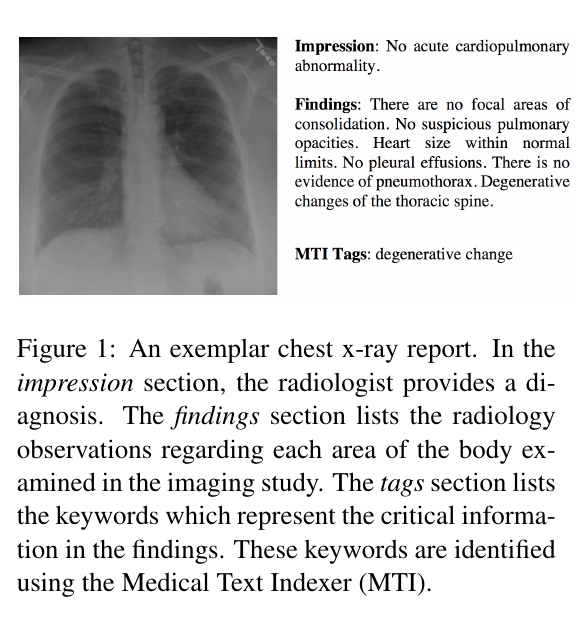
\includegraphics[scale=0.5]{images/baoyu_jing_report}
\par\end{centering}
\caption{Sample report from IU X-ray}

\end{figure}


\subsection{Methods and Architecture}

An image is divided into regions, and a CNN encoder is used to learn
visual features for these patches. These features are fed into a \emph{multi-label
classifier}, from which tags are predicted. These tags are transformed
into \emph{semantic feature vectors }by a custom embedding. Both visual
and semantic features are fed into the co-attention module, which
produces a combined \emph{context vector, }which \textbf{simultaneously
captures the visual and semantic information of this image.} 

The decoding and caption generation process is performed by the hierarchical
LSTM, which leverages the compositional structure of a medical report
(each sentence focusing on one specific topic). The \emph{sentence
LSTM}, using the context vector, first generates a sequence of high-level
topic vectors representing sentences. Each one is passed to the \emph{word
LSTM,} which then generates a sentence for each topic vector. The
number of sentences or topic vectors to be generated is regulated
by the \emph{stop control}.

\begin{figure}
\begin{centering}
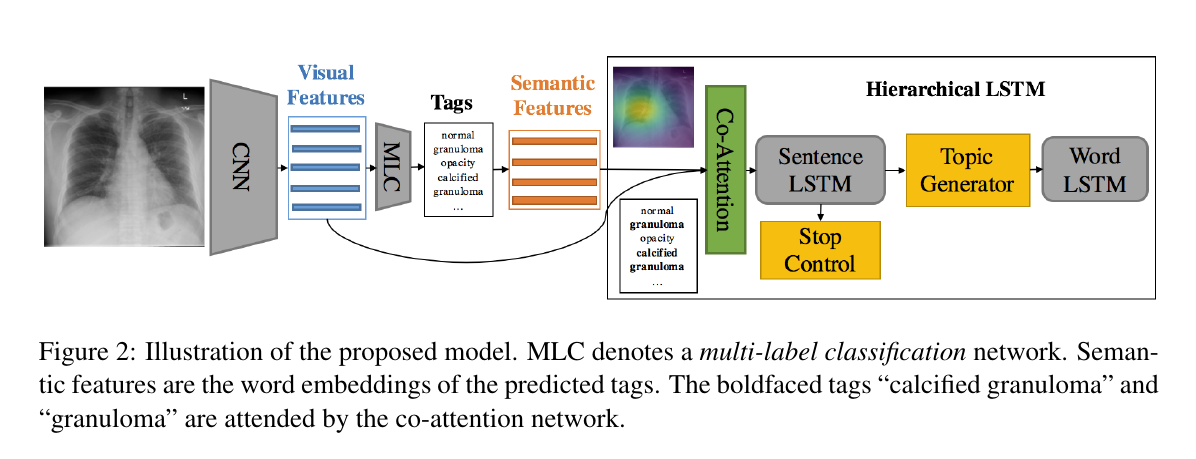
\includegraphics[scale=0.5]{images/baoyu_jing_architecture}
\par\end{centering}
\caption{Architecture}
\end{figure}


\subsubsection{Tag prediction}

This is treated as a multi-label classification task. Given an image
$I$, visual features $\left\{ \boldsymbol{v}_{n}\right\} _{n=1}^{N}\in\mathbb{R}^{D}$
are extracted from the CNN encoder, and fed to a \emph{multi-label
classification }(MLC) network, which then generates a probability
distribution over the $L$ tags
\[
\boldsymbol{p}_{I,\text{pred}}\left(\boldsymbol{l}_{i}=1\;|\;\left\{ \boldsymbol{v}_{n}\right\} _{n=1}^{N}\right)\propto\exp\left(\text{MLC}_{i}\left(\left\{ \boldsymbol{v}_{n}\right\} _{n=1}^{N}\right)\right)
\]
\\
where $\boldsymbol{l}\in\mathbb{R}^{L}$ is a binary tag vector, each
component representing the presence or absence of the corresponding
tag.\\
Finally, the embeddings of the $M$ most likely tags $\left\{ \boldsymbol{a}_{m}\right\} _{m=1}^{M}$
are used as \textbf{semantic features. }

\subsubsection{Co-Attention}

Visual attention does not provide sufficient high-level semantic information,
which the tags can always provide. A co-attention mechanism can simultaneously
attend to visual and semantic modalities.

In the sentence LSTM at time step $s$, the joint context vector \textbf{$\text{\textbf{ctx}}^{(s)}\in\mathbb{R}^{C}$
}is generated by a co-attention network $f_{\text{co-att}}\left(\left\{ \boldsymbol{v}_{n}\right\} _{n=1}^{N},\left\{ \boldsymbol{a}_{m}\right\} _{m=1}^{M},\boldsymbol{h}_{\text{sent}}^{(s-1)}\right)$,
with $\boldsymbol{h}_{\text{sent}}^{(s-1)}\in\mathbb{R}^{H}$ being
the previous hidden state. The co-attention network $f_{\text{co-att}}$
uses a single feedforward layer to compute separate soft visual and
semantic attentions
\begin{align*}
\alpha_{\vec v,n} & \propto\exp\left(\vec W_{\vec v_{\text{att}}}\vec v_{n}+\vec W_{\vec v,\vec h}\vec h_{\text{sent}}^{(s-1)}\right)\\
\alpha_{\vec a,m} & \propto\exp\left(\vec W_{\vec a_{\text{att}}}\vec a_{m}+\vec W_{\vec a,\vec h}\vec h_{\text{sent}}^{(s-1)}\right)
\end{align*}
\\
The visual and semantic context vectors 
\begin{align*}
\vec v_{\text{att}}^{(s)} & =\sum_{n=1}^{N}\alpha_{\vec v,n}\vec v_{n}\\
\vec a_{\text{att}}^{(s)} & =\sum_{m=1}^{M}\alpha_{\vec a,m}\vec a_{m}
\end{align*}
\\
These context vector may be combined by concatenation followed by
a fully connected layer:

\[
\vec{ctx}^{(s)}=\vec W_{\text{fc}}\left[\vec v_{\text{att}}^{(s)};\vec a_{\text{att}}^{(s)}\right]
\]


\subsubsection{Sentence LSTM}

A single LSTM layer whose input is the joint context vector $\vec{ctx}^{(s)}$
and generates a topic vector $\vec t\in\mathbb{R}^{K}$as long as
the stop control allows it to. 

\paragraph{Topic generator}

Deep output layer (LSTM + multi-layer feedforward) 
\[
\vec t^{(s)}=\tanh\left(\vec W_{\vec t,\vec h}\vec h_{\text{sent}}^{(s)}+\vec W_{\vec t,\vec{ctx}}\vec{ctx}^{(s)}\right)
\]


\paragraph{Stop control }

Deep output layer for the continuation of the sentence LSTM. The layer
takes the previous and current hidden states and produces a distribution
over $\left\{ \text{STOP}=1,\text{CONTINUE}=0\right\} $, $p_{\text{stop}}^{(s)}$
\begin{align*}
p\left(\text{STOP}\;|\;\vec h_{\text{sent}}^{(s-1)},\vec h_{\text{sent}}^{(s)}\right) & \propto\exp\left\{ \text{\ensuremath{\vec W_{\text{stop}}\tanh\left(\vec W_{\text{stop},s-1}\vec h_{\text{sent}}^{(s-1)}+\vec W_{\text{stop},s-1}\vec h_{\text{sent}}^{(s)}\right)}}\right\} 
\end{align*}
\\
This stopping probability is then compared with a predefined threshold.

\subsubsection{Word LSTM}

For each topic vector, the words in the sentence are generated by
the \emph{word LSTM.} Its first and second inputs are the topic vector
$\vec t$ and a $\text{START}$ token, then followed by the rest of
the words \citep{krause2016hierarchical}. Each hidden state $\vec h_{\text{word}}\in\mathbb{R}^{H}$
is directly used to predict the distribution over words:
\[
p\left(\text{word}\;|\;\vec h_{\text{word}}\right)\propto\exp\left(\vec W_{\text{out}}\vec h_{\text{word}}\right)
\]


\subsubsection{Parameter learning}

Each training example is a tuple $\left(I,\text{\ensuremath{\vec l},\ensuremath{\vec w}}\right)$,
with $\vec w$ being the paragraph, with $S$ sentences, each with
$T_{S}$ words (ground truth). 
\begin{enumerate}
\item The MLC predicts the tag distribution $\vec p_{I,\text{pred}}$. Its
ground truth may be computed by $\vec p_{I}=\vec l/\left\Vert \vec l\right\Vert _{1}$.
Thus, the training loss for this task is the cross-entropy between
both distributions $\ell_{\text{tag}}$.
\item The sentence LSTM is unrolled for $S$ steps, producing that number
of topic vectors $\vec t^{(s)}$ and stop distributions $p_{\text{stop}}^{(s)}$.
For each sentence, this stop probability is compared with the indicator
$I\left\{ s=S\right\} $, which evaluates to $0\;\text{[CONTINUE]}$,
until $s=S$, when it evaluates to $1\;\text{[STOP]}$ (that is, a
kronecker delta $\delta_{sS}$). The cross entropy between them is
the loss $\ell_{\text{sent}}$.
\item The $S$ topic vectors are fed to the word LSTM to generate $\vec w_{s,t}$
words. The training loss for each word is the cross entropy $\ell_{\text{word}}$
between the ground truth word $w_{s,t}$ and the predicted word distribution
$p_{s,t}$.
\end{enumerate}
Thus, the overall training loss is 
\begin{align*}
\ell\left(I,\text{\ensuremath{\vec l}},\vec w\right) & =\lambda_{\text{tag}}\ell_{\text{tag}}\\
 & +\lambda_{\text{sent}}\sum_{s=1}^{S}\ell_{\text{sent}}\left(p_{\text{stop}}^{(s)},I\left\{ s=S\right\} \right)\\
 & +\lambda_{\text{word}}\sum_{s=1}^{S}\sum_{t=1}^{T_{S}}\ell_{\text{word}}\left(p_{s,t},w_{s,t}\right)
\end{align*}

Furthermore, and attention regularization loss \citep{xu2015attend}
for both visual $\boldsymbol{\alpha}\in\mathbb{R}^{N\times S}$ and
semantic $\boldsymbol{\beta}\in\mathbb{R}^{M\times S}$ attention
coefficients. This regularization encourages the model to pay equal
attention over different image regions and tags. 
\[
\ell_{\text{reg}}=\lambda_{\text{reg}}\left[\sum_{n=1}^{N}\left(1-\sum_{s=1}^{S}\alpha_{n,s}\right)^{2}+\sum_{m=1}^{M}\left(1-\sum_{s=1}^{S}\beta_{m,s}\right)^{2}\right]
\]


\section{Evaluation of text generation: A survey \citep{reviewmetrics2020}}

Surveys evaluation methods for Natural Language Generation (NLG) that
may be classified as 
\begin{itemize}
\item Human-centric evaluation
\item Automatic metrics
\item Machine-learned evaluation
\end{itemize}

\subsection{Introduction}

NLG evaluation is challenging mainly because many NLG tasks are open-ended
(\emph{i.e. }multiple valid answers for a task), so human evaluation
remains the gold standard. 

NLG techs range from template-based systems to machine learned systems
that have a complex understanding of human grammar. There has been
a paradigm shift from earlier template-based models using statistical
methods and expert knowledge to unsupervised learning of representations
from large textual corpora by using DNN models. This shift crosses
through RNNs, (LSTM, GRU), word2vec, GloVe, and sequence-to-sequence
by encoder-decoder architecture. These latter models' weakness of
capturing long-range dependencies motivates the development of \emph{attention
networks} and \emph{pointer networks}. The transformer architecture
combines both encoder-decoder with a self-attention mechanism. 

Neural models have been applied to many NLG tasks:
\begin{itemize}
\item summarization: documents, query-focused or generic, for news articles,
meetings, etc
\item machine translation
\item dialog systems: goal-oriented or chit-chat
\item question generation
\item long text generation: story, news, poem
\item data-to-text generation: \emph{e.g.} table summarization
\item \textbf{caption generation from non-text input:} tables, images or
sequences of video frames 
\end{itemize}
\begin{quote}
\emph{``Nevertheless, training a powerful language model relies on
evaluation metrics that can measure the model quality from different
perspectives. For instance, it is imperative to build evaluation methods
that can determine whether a text is generated by a human or a machine
to prevent any potential harm. Similarly, evaluating the generated
text based on factual consistency has recently drawn attention in
the NLG field. It is concerning that neural language models can generate
open-ended texts that are fluent but not grounded in real-world knowledge
or facts, such as fake news. The situation is particularly alarming
if the generated reports or news are related to the well-being of
humankind, such as summaries of health reports.''}
\end{quote}

\subsubsection{Outline}
\begin{itemize}
\item \textbf{Human-centric Evaluation: }\emph{humans as judges. }Task-specific. 
\item \textbf{Untrained Automatic Metrics: }Most commonly used, compared
model outputs to references with metrics based on string overlap,
content overlap, string distance or lexical diversity.
\item \textbf{Machine-learned Metrics: }models that can be viewed as digital
judges that simulate human judges.
\end{itemize}

\subsection{Human-Centric Evaluation Methods}

The ultimate goal of NLG is to generate text that is valuable to people.
\\
Human evaluations pose several challenges: expensive and time-consuming
to run, especially for tasks that require domain expertise. There
is also a lack of consistency in how these evaluations are run, which
prevents reproducibility and comparing across systems. 

\subsubsection{Intrinsic Evaluation}

An \emph{intrinsic evaluation} asks people to evaluate the quality
of generated text, either overall or along some specific dimension
(e.g., fluency, coherence, correctness, etc.). This may be done by
showing each text individually and asking for an assessment by binary
(good/bad) or Likert/sliding scale. However, these judgments can be
inconsistent and comparing these results is not straightforward. 

Another approach to directly compare to baselines model variants,
or human generated texts: evaluations can be performed by selecting
or ranking generated texts. This captures models' relative quality
but not absolute. This can be solved by asking judges to indicate
how much better the chosen text is over alternatives. Comparison-based
approaches can become prohibitively expensive (by number of matchups),
though this may be somewhat mitigated.

Some dimensions of human evaluation include:
\begin{itemize}
\item \emph{Adequacy: “how much of the meaning expressed in the gold-standard
translation or source is also expressed in the target translation''}
\item \emph{Fluency: }quality of text without taking the source into account,
accounting for grammar, spelling, choice of words, style, etc.
\item \emph{Factuality: }important in tasks that require the generated text
to accurately reflect facts described in the context (many neural
NLG models ``hallucinate'' information)
\item Misc: \emph{commonsense, logicality, coherence or consistency}
\end{itemize}
Other dimensions focus on \emph{how }the text is being said, without
context:
\begin{itemize}
\item \emph{Grammaticality}
\item \emph{Style, formality }or \emph{tone}
\item \emph{Typicality: }how often do you expect to see text that looks
like this?
\item \emph{Redundancy}
\end{itemize}

\printbibliography

\end{document}
